\documentclass{article}
% --- watermark (auto-inserted) ---
\usepackage{xcolor}
\usepackage{xfp}% \fpeval; in the kernel since 2022, harmless on older LaTeX
\usepackage{draftwatermark}
\newlength{\watermarkTextWidth}
\AddToHook{begindocument/end}{%
  \SetWatermarkText{\normalfont Generated by The Agentic Scientist}%
  \SetWatermarkFontSize{10pt}%
  \SetWatermarkLightness{0.85}%
  \settowidth{\watermarkTextWidth}{\normalfont\fontsize{10pt}{12pt}\selectfont Generated by The Agentic Scientist}%
  \edef\watermarkScale{\fpeval{0.8 * sqrt(\paperwidth**2 + \paperheight**2) / \watermarkTextWidth}}%
  \edef\watermarkAngle{\fpeval{atand(\paperheight/\paperwidth)}}%
  \SetWatermarkScale{\watermarkScale}%
  \SetWatermarkAngle{\watermarkAngle}%
}
% --- end watermark ---
 % For LaTeX2e
\usepackage{paper,times}

\usepackage{hyperref}
\usepackage{url}
\usepackage{amsmath,amssymb}
\usepackage{booktabs}
\usepackage{graphicx}

\newcommand{\score}{\mathrm{Score}}

\title{Gated Weighted-Mondrian Conformal Sets for Softmax Outputs: A Multi-Axis Reliability Evaluation on Synthetic Simplex Families}
\author{Anonymous authors}

\begin{document}
\maketitle

\begin{abstract}
Softmax outputs are compositions: non-negative vectors summing to one. Conformal prediction turns them into label sets with a finite-sample marginal coverage guarantee, but marginal coverage says little about reliability for particular classes, confidence strata, or shifted data. We study a split-conformal procedure that combines Mondrian (class- or confidence-bin-conditional) calibration of the least-ambiguous-set score with a gated, cross-fitted domain-classifier reweighting step that reduces exactly to the unweighted procedure when no shift is detected. We evaluate it under a fixed, evaluator-owned protocol on synthetic softmax families: a composite score combining one-sided marginal under-coverage, worst-slice under-coverage, and set-size ratio, plus negative controls. On sealed final data (five seeded runs, no failed episodes, all controls passed) the procedure scores 0.8416 against 0.8029 for the best of four standard split-conformal baselines; the paired margin is 0.0387 (bootstrap 95\% interval 0.0274--0.0499). Residual under-coverage remains on shifted cases (0.0536) and worst slices (0.0675). The result is conditional on the declared synthetic families; baseline identities, per-case results and real-data behaviour are unavailable.
\end{abstract}

\section{Introduction}
Many predictors return a composition: a vector of non-negative entries summing to one, such as a classifier's softmax probabilities. Users of such outputs need to know when the associated uncertainty statement can be trusted. Conformal prediction converts a score function and a held-out calibration set into prediction sets whose marginal coverage is at least $1-\alpha$ under exchangeability, in finite samples and without distributional assumptions. In practice, however, three questions that matter to a user are not answered by the marginal guarantee: does coverage hold within classes or confidence strata, does it survive a change in the input distribution, and is it achieved with sets that are small enough to be informative? Our motivation is that a method tuned for one question may do worse on another, so reporting only average coverage and set size can hide such differences; conditional-coverage and efficiency work \citep{Gibbs2023ConformalPW,Ding2023ClassConditionalCP,Kiyani2024LengthOI} makes the individual questions concrete.

This paper takes the evaluation protocol as its first-class object. We adopt a single evaluator-owned protocol on synthetic softmax families that scores a set-valued predictor on three axes at once (one-sided marginal under-coverage, worst-slice under-coverage, and set-size ratio) and that adds negative controls whose expected behaviour is fixed before scoring. Within this protocol we ask:
\emph{does a Mondrian least-ambiguous-set conformal procedure with a gated, cross-fitted domain-classifier reweighting step achieve a better composite reliability score than standard split-conformal baselines, and where do its guarantees visibly stop holding?}

The answer we can support is conditional. On sealed final data the studied procedure obtains a higher composite score than the best of four evaluator-implemented baselines, with a paired margin whose bootstrap interval excludes zero; it also shows a small one-sided marginal under-coverage gap (0.0017) on exchangeable cases. At the same time, the sealed metrics show non-trivial residual under-coverage on shifted cases and on worst slices, and the retained artifacts do not allow us to say which baseline was best, which cases drive the residual gaps, or whether the result extends beyond the declared families.

\paragraph{Contributions.}
(i) We write down the three-axis protocol in reader-checkable form, including the loss, the slice definitions, the negative controls and the validity conditions, and derive simple properties relevant to interpreting scores (for example, that the full prediction set scores exactly 0.75 and that the one-sided gap metrics do not penalise over-coverage).
(ii) We specify one concrete procedure, composed from known pieces (Mondrian calibration, likelihood-ratio weighted conformal thresholds, a held-out gate), and state which of its properties are exact and which are only approximate when the weights are estimated.
(iii) We report a sealed final comparison with uncertainty and decompose the residual loss into its marginal, slice and size components.
(iv) We delimit scope: the evidence concerns synthetic families, one sealed evaluation, and one aggregated baseline comparison. We make no claim of a new theorem or of a compositional-geometry method; the procedure operates on summary features of the probability vector.

\begin{figure}[htbp]
\centering
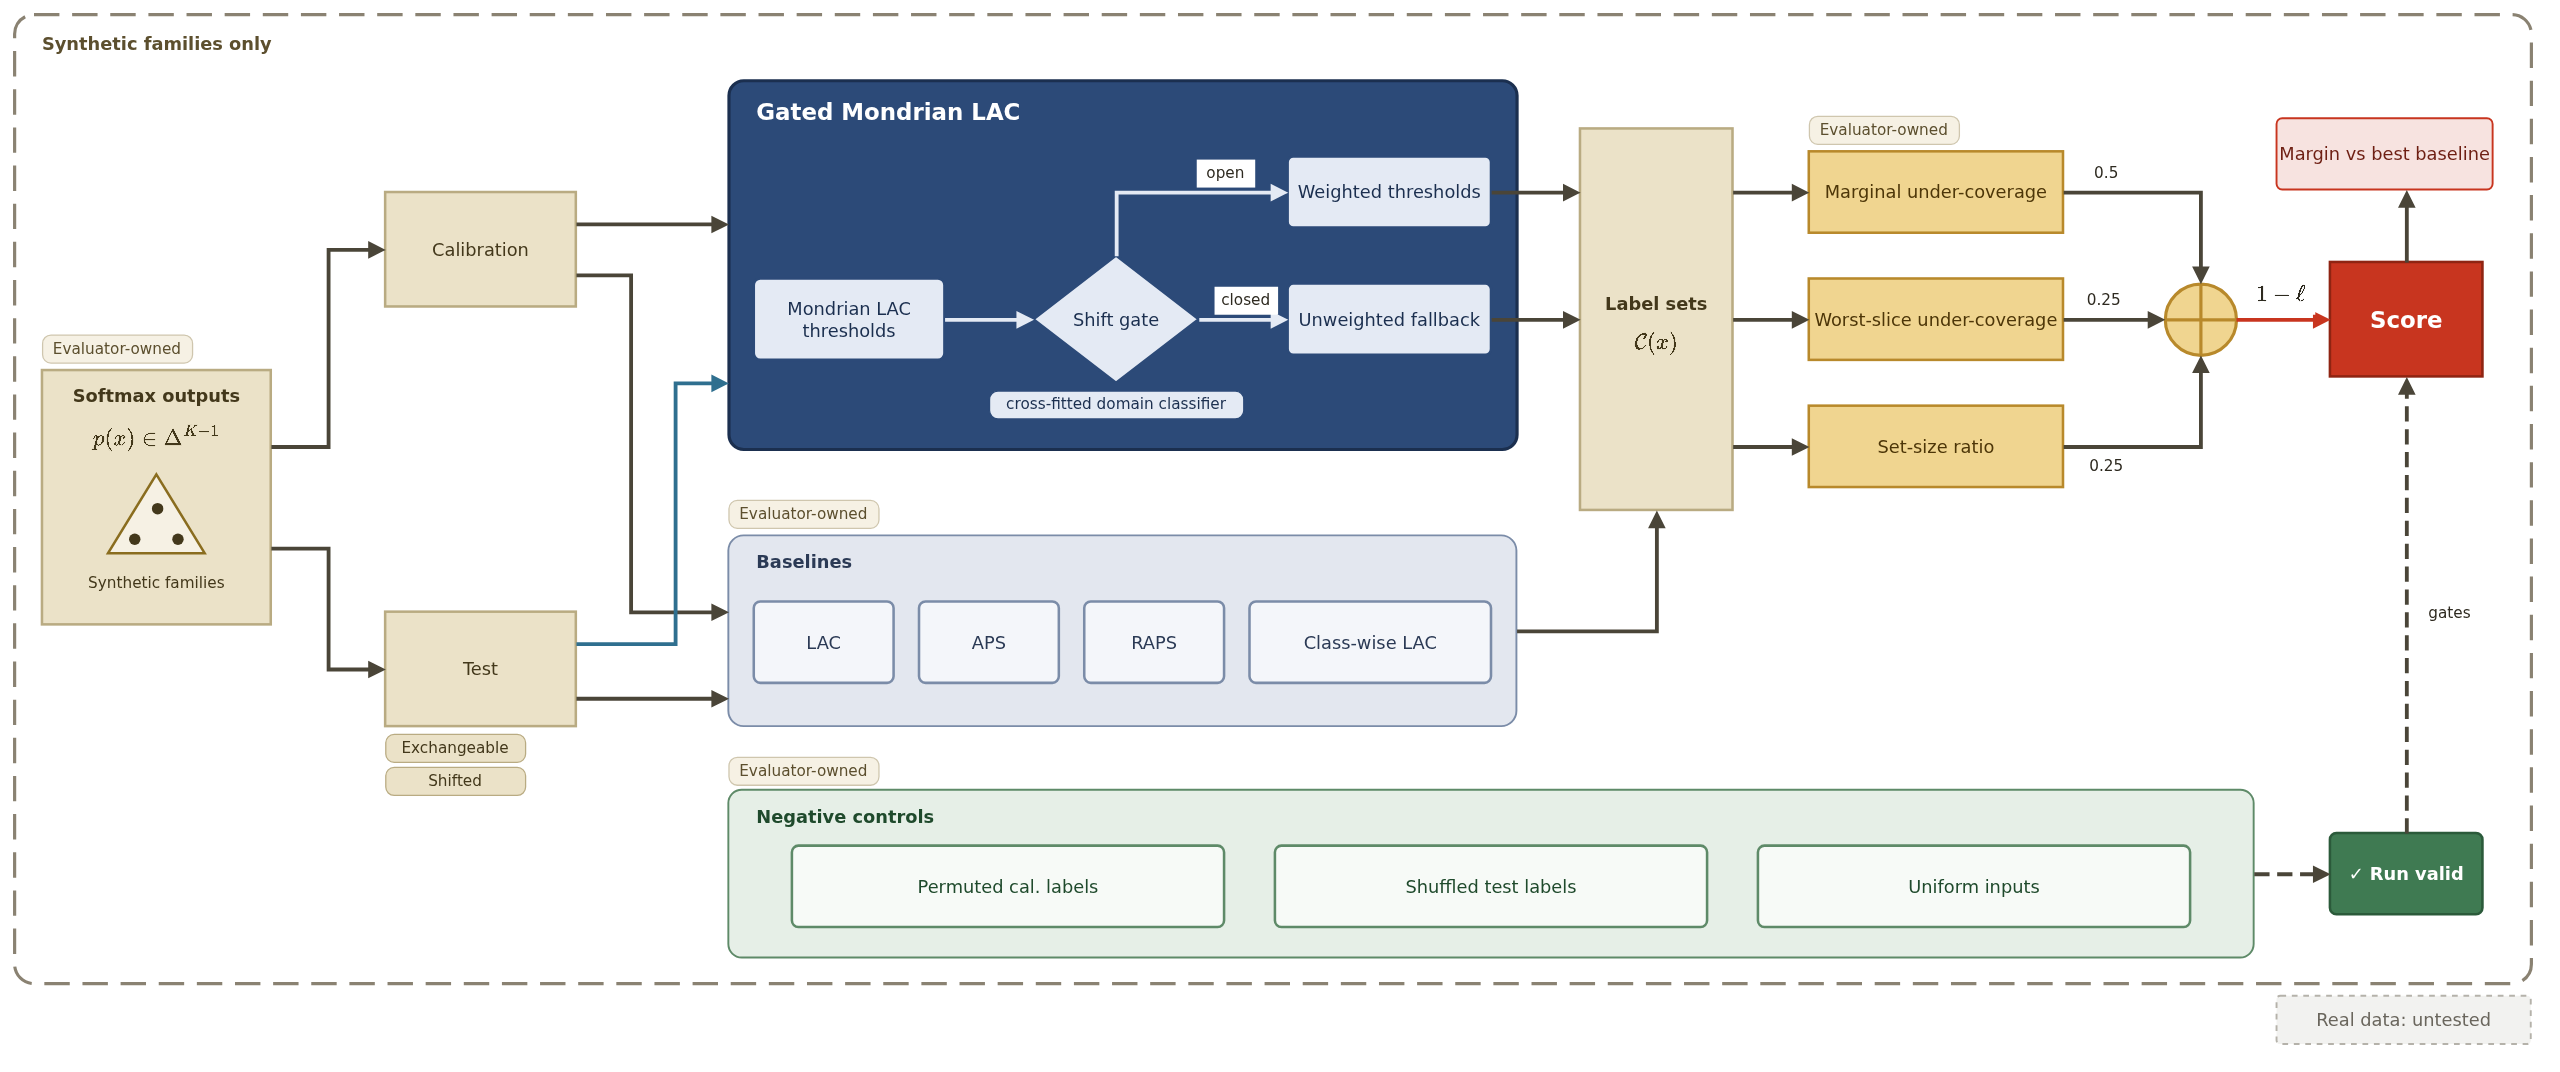
\includegraphics[width=\textwidth]{figures/protocol_overview.png}
\caption{Evaluation protocol at a glance. Simplex-valued softmax outputs from evaluator-generated synthetic families are split into calibration and test parts. The studied procedure (Mondrian LAC with gated domain-classifier weighting) and four evaluator baselines (LAC, APS, RAPS, class-wise LAC) produce label sets, which are scored on three axes (marginal under-coverage with weight 0.5, worst-slice under-coverage 0.25, set-size ratio 0.25) and checked by negative controls. Scope is limited to the declared synthetic families.}
\label{fig:overview}
\end{figure}

\section{Related Work}\label{sec:related}
\paragraph{Foundations and classification scores.}
Split conformal prediction uses a held-out calibration set and retains finite-sample marginal coverage under exchangeability \citep{Vovk2005Algorithmic,Lei2018Distribution}; Mondrian conformal prediction applies the same rank argument within partition cells \citep{Vovk2005Algorithmic}. For classifiers, the least-ambiguous-set construction thresholds the softmax mass of each label \citep{Sadinle2019Least}, adaptive prediction sets accumulate sorted probability mass with randomisation \citep{Romano2020Classification}, and a regularised variant penalises large ranks to shrink sets on many-class problems \citep{Angelopoulos2020Uncertainty}. These are our comparators (Section~\ref{sec:method}).

\paragraph{Conditional validity.}
Several works address conditional-coverage guarantees beyond the marginal guarantee, including conditional guarantees for conformal prediction \citep{Gibbs2023ConformalPW} and coverage beyond class- and covariate-conditional notions \citep{Bairaktari2025KandinskyCP}. Conditional conformal prediction has been proposed for bias reduction \citep{Löfström2015BiasRT}, and recent work addresses class-conditional coverage with many classes \citep{Ding2023ClassConditionalCP}, conformal prediction for long-tailed classification \citep{Ding2025ConformalPF}, and class-wise coverage via augmented label rank calibration \citep{Shi2024ConformalPF}. Group-conditional thresholds have also been learned by quantile regression \citep{Melki2023GroupConditionalCP}, trust scores have been used to improve conditional coverage \citep{Kaur2025ConformalPS}, and coverage conditional on a selection event has been studied \citep{Jin2024ConfidenceOT}. Our procedure uses the simplest member of this family, Mondrian groups defined by label or by confidence bin, and we examine a quantile-regression variant only as a development-time comparison.

\paragraph{Efficiency and the classifier.}
Set size is a second axis: length-optimal conformal prediction \citep{Kiyani2024LengthOI}, classifier adaptation for efficient sets \citep{Liu2024CAdapterAD}, the interaction between temperature scaling and conformal sets \citep{Dabah2024OnTS}, and the quality of foundation-model features as conformal predictors \citep{Fillioux2024AreFM} all bear on how small a valid set can be. Related variants combine conformal prediction with Monte Carlo prediction \citep{Bethell2023RobustUQ} and interpretable networks \citep{Huang2024CONFINECP}.

\paragraph{Other output types and settings.}
Conformal methods exist for time series \citep{Xu2022ConformalPS}, ordinal labels \citep{Chakraborty2024DistributionfreeCP}, heteroskedastic regression with conditional validity \citep{Dewolf2023ConditionalVO}, multivariate residuals \citep{Braun2025MultivariateSR}, epistemic-uncertainty settings \citep{Javanmardi2025OptimalCP} and connections to scenario optimisation \citep{O'Sullivan2025BridgingCP}. Applied treatments of conformal classifiers appear in clinical imaging and histopathology \citep{Cina2026QuantifyingCC,Gelvez2025ConformalPF}. We describe these works only by title and venue.

\paragraph{Distribution shift.}
Under covariate shift, exchangeability fails. If the density ratio is known, reweighting the calibration scores by it and giving the test point its own weight restores marginal coverage \citep{Tibshirani2019Conformal}; estimating the ratio with a calibration-versus-test classifier makes the guarantee approximate. Our gated step follows this recipe with an explicit unweighted fallback.

\paragraph{Positioning.}
Our contribution is neither a new conformal score nor a new guarantee. It is a combined reading of one evaluation protocol and one composition of established components (Mondrian calibration, likelihood-ratio weighted conformal thresholds, and a held-out gate), with sealed evidence and an explicit account of where it fails. Compositional-data analysis in the sense of log-ratio geometry \citep{Aitchison1982Statistical} motivates the framing (outputs live on the simplex), but the procedure studied here does not use log-ratio coordinates for its prediction sets.

\section{Method}\label{sec:method}
\subsection{Problem setup and evaluation target}\label{sec:setup}
Let $p(x)\in\Delta^{K-1}$ be the softmax output of a fixed $K$-class predictor, with $y\in\{1,\dots,K\}$. A conformal procedure receives $n_{\mathrm{cal}}$ labelled calibration pairs $(p_i,y_i)$, the level $\alpha$, and $n_{\mathrm{test}}$ unlabelled test vectors, and returns a set $\mathcal C(x)\subseteq\{1,\dots,K\}$ for each test vector. The evaluator owns the data: logits are $z=\epsilon+s\,d\,e_y+\beta\log\pi_{\mathrm{cal}}$ with $\epsilon\sim\mathcal N(0,I_K)$, signal strength $s$, a log-normal heteroscedastic multiplier $d$ on the true-class signal, a prior tilt $\beta$, and temperature scaling before the softmax; the class prior is balanced or long-tailed. Test data may differ from calibration data through the class prior and a signal-strength multiplier (``shifted'' cases); otherwise a case is exchangeable. The declared range is $2\le K\le 100$, $n_{\mathrm{cal}}\le 2000$, $n_{\mathrm{test}}\le 4000$ in the search-time evaluator source; the sealed final case manifest (families, $K$, $\alpha$, sample sizes) is not retained and is therefore unknown to us.
% @evidence[[source_evidence/evaluator/evaluate.py#gen_split]]

\subsection{Composite reliability score}
For one episode with set indicator $\mathcal C(x_j)$ on $n$ test points, let $\mathrm{cov}$ be empirical coverage, $\rho=\frac1{nK}\sum_j|\mathcal C(x_j)|$ the set-size ratio, and $g_{\mathrm{m}}=\max(0,1-\alpha-\mathrm{cov})$ the one-sided marginal gap. The worst-slice gap $g_{\mathrm{s}}$ is the largest one-sided coverage shortfall over slices with at least 30 test points: classes when $K\le10$, and strata of set size and of maximum probability (quartiles) when $K>10$. The episode loss and score are
\begin{equation}
\ell=0.5\,\mathrm{clip}_{[0,1]}(g_{\mathrm m}/\alpha)+0.25\,\mathrm{clip}_{[0,1]}(g_{\mathrm s})+0.25\,\mathrm{clip}_{[0,1]}(\rho),\qquad \score=1-\overline{\ell},
\label{eq:loss}
\end{equation}
where $\overline\ell$ averages over seeds within a case and with equal weight over cases. Two properties follow directly from Eq.~\eqref{eq:loss}. First, the full set has $g_{\mathrm m}=g_{\mathrm s}=0$ and $\rho=1$, so it scores exactly $0.75$ on every case; any useful procedure must beat this by shrinking sets without opening coverage gaps. Second, the gaps are one-sided: over-coverage is penalised only through $\rho$, so a small gap does not show that coverage is tight. Shift-case coverage enters $\score$ through the same terms, but the shift gap is reported as a descriptive metric and is not a validity condition.
% @evidence[[source_evidence/evaluator/evaluate.py#score_sets]]

\subsection{Baselines, negative controls and validity conditions}
The evaluator scores four standard split-conformal baselines on identical data with the same loss, drawn from the score families of Section~\ref{sec:related}: LAC \citep{Sadinle2019Least} (threshold on $1-p_y$), APS \citep{Romano2020Classification} (randomised cumulative-mass score), RAPS \citep{Angelopoulos2020Uncertainty} (APS with a rank penalty, $\lambda=0.01$, regularisation start $\min(5,\max(1,\lfloor K/5\rfloor))$) and class-wise LAC (LAC calibrated per label). Exact implementations are those of the evaluator source, not re-derived from the cited papers. Uncalibrated top-mass, full-set and argmax-only sets are implemented as trivial references. The reported baseline score is that of the best of the four baselines under the aggregated score; the margin is $\score_{\mathrm{proc}}-\score_{\mathrm{best}}$, and its 95\% interval is the 2.5--97.5 percentile of 2000 bootstrap resamples of the per-seed paired differences within each case, averaged with equal weight over cases. The interval therefore reflects seed-to-seed variation inside the evaluated cases and not variation across case designs.

In the search-plane evaluator source, three negative controls are defined, each run on one case and seed: (C1) permuted calibration labels, where sets must inflate (size ratio at least $1.5\times$ the matched case or at least $0.9$); (C2) shuffled test labels, where coverage must not exceed chance by more than a $3\sigma$ tolerance and must be well below matched coverage or sets near full; (C3) uniform probability inputs, where coverage must be at least the target minus a tolerance and mean set size at least $(1-\alpha)K-1$; this check is one-sided, so over-coverage is not penalised by it. The number of final-plane controls is not retained; only a controls-passed fraction of 1.0 is. A run is valid only if no episode fails, all controls pass, calibration and test data are content-hash disjoint (and, for the final plane, disjoint from the search data), and exchangeable cases do not under-cover by more than a $3\sigma$ finite-sample tolerance.
% @evidence[[source_evidence/evaluator/evaluate.py#control_verdicts]]

\subsection{Statistical background and what it predicts}
\paragraph{Marginal and Mondrian validity.}
With exchangeable calibration and test points and continuous scores, split conformal with threshold equal to the $k$-th smallest of $n$ calibration scores, $k=\lceil (n+1)(1-\alpha)\rceil$, covers with probability $k/(n+1)\in[1-\alpha,\,1-\alpha+1/(n+1))$, and coverage conditional on the calibration set follows a $\mathrm{Beta}(k,n+1-k)$ law \citep{Vovk2005Algorithmic,Lei2018Distribution}. Applying the same rank argument within each cell of a partition $G(x,y)$ yields cell-conditional coverage (Mondrian calibration, \citealt{Vovk2005Algorithmic}); with $G$ equal to the label this is class-conditional coverage, and with $G$ a function of $x$ alone it is conditional on the stratum. These are textbook statements \citep{Vovk2005Algorithmic} and we do not claim them as new.

\paragraph{Proposition (Mondrian coverage; textbook).}
Let $G$ be a partition cell function of $(x,y)$ and let the calibration scores of cell $g$ be $s_1,\dots,s_{n_g}$, exchangeable with the test score $s_{\mathrm{new}}$ conditional on the test point lying in cell $g$, with no ties. Take $q_g$ equal to the $k_g$-th smallest calibration score, $k_g=\lceil(n_g+1)(1-\alpha)\rceil$. Then $\Pr(s_{\mathrm{new}}\le q_g\mid G=g)\ge1-\alpha$.
\emph{Proof sketch.} By exchangeability the rank of $s_{\mathrm{new}}$ among the $n_g+1$ scores is uniform on $\{1,\dots,n_g+1\}$. The event $s_{\mathrm{new}}\le q_g$ holds exactly when this rank is at most $k_g$, which has probability $k_g/(n_g+1)\ge1-\alpha$; ties only increase the probability. $\square$
For $G=y$ the cell is observable only at calibration time, and the set $\{k:1-p_k(x)\le q_k\}$ covers the true label $y$ with class-conditional probability at least $1-\alpha$ because the event is $\{s(x,y)\le q_y\}$. For $G$ a function of $x$ alone the cell is known at prediction time. The guarantee is conditional on the cell and does not extend to other partitions: when $K>10$ the evaluator's slices (strata of set size and of maximum probability in quartiles) differ from the Mondrian confidence bins used here. The implemented thresholds also depart from the proposition: lowering $\alpha_g$ by a margin can only raise $q_g$, but shrinking $q_g$ toward the pooled threshold can lower it, so the implemented procedure has no exact cell-conditional guarantee, only the exact quantile at level $\alpha_g$ does. The data-dependent gate below is \emph{not} covered by this argument: it uses unlabelled calibration and test features, it treats the two groups asymmetrically, and we have not derived a guarantee for the draws on which it activates under exchangeability. We therefore use the proposition only as background for the fallback branch.

\paragraph{Weighted calibration under covariate shift.}
If test inputs follow density ratio $w(x)$ with respect to calibration inputs and $w$ is known, placing the test point's weight at $+\infty$ in the weighted empirical distribution of calibration scores restores marginal coverage \citep{Tibshirani2019Conformal}; with an estimated $w$ the guarantee is only approximate. Our procedure estimates $w$ with a classifier on summary features, so we treat the weighted branch as a heuristic correction whose benefit has to be measured, not as a guaranteed one.

\paragraph{Why a one-sided loss favours a small margin.}
Under the normal approximation to the Beta law, calibration-induced coverage is $C\approx\mathcal N(\mu,\sigma^2)$ with $\sigma^2\approx\alpha(1-\alpha)/(n+2)$ and $\mu\ge1-\alpha$. The expected one-sided shortfall is $\sigma\,f(\delta)$ with $f(\delta)=\varphi(\delta)-\delta(1-\Phi(\delta))$ and $\delta=(\mu-(1-\alpha))/\sigma$. An exact-level quantile has $\delta\approx0$ and $f(0)=0.399$, whereas shifting the level by $0.7\sigma$ gives $f(0.7)=0.143$, about 36\% of the unmargined value, at the price of larger sets. This is the motivation for the variance-aware margins used below (multipliers 0.7 pooled, 0.6 per group). It is a heuristic derivation about calibration noise only; we have no unmargined ablation, so it is not checked experimentally here.
% @evidence[[derived/derived_stats.json#margin_constants]]

\subsection{Design rationale and hypotheses}
The procedure is built around three expectations, each tied to one component. \textbf{H1}: grouping calibration by label (small $K$) or confidence bin (large $K$) should shrink worst-slice under-coverage relative to pooled calibration, because it makes the coverage guarantee hold within the evaluator's slices when those coincide with the groups. \textbf{H2}: a gated, cross-fitted density-ratio correction should reduce marginal under-coverage on shifted cases, while a gate that stays closed leaves exchangeable behaviour and the negative controls untouched. \textbf{H3}: group-indicator quantile-regression thresholds could further reduce worst-slice gaps when the groups are overlapping. The retained evidence addresses these only partially: H1 is not isolated (no pooled-versus-Mondrian pair of otherwise identical configurations was retained, and baseline identities are unknown); H2 is supported only descriptively by the development comparison V1 versus V2 on three seeds, while the sealed shift-case gap is a residual of the frozen procedure with no unweighted or baseline counterpart and so does not test H2; H3 is untestable from V3 because V3 coincides with V2. The aim of the sealed evaluation is thus the narrower statement of Section~\ref{sec:results} about the composite score, not a verification of each hypothesis.

\subsection{Studied procedure}
\paragraph{Mondrian LAC.}
The score of label $k$ is $1-p_k(x)$ (LAC). For $K\le10$ the Mondrian groups are the labels, because the evaluator's slices are classes; for $K>10$ they are confidence bins of the maximum probability (at most 10 equal-mass bins, at least 80 calibration rows each), a function of $x$ alone. Each group's threshold is the finite-sample conformal quantile at level $\alpha_g=\alpha-z\sqrt{\alpha(1-\alpha)(1/n_g+k_g/M)}$ with $z=0.6$ per group and $0.7$ for the pooled threshold, where $M$ is the number of test rows and $k_g$ the number of groups; group thresholds are shrunk toward the pooled threshold with weight $n_g/(n_g+20)$, and groups too small for a finite quantile use the pooled value. The set is $\{k: 1-p_k(x)\le q_{g}\}$.
% @evidence[[source_evidence/V2/program.py#mondrian_conformal_quantile]]

\paragraph{Gated cross-fitted weighting.}
Each probability vector is mapped to five summary features (logit of the top probability, top-two log ratio, normalised entropy, mean top-five log probability minus the top log probability, log normalised Gini impurity), standardised with calibration moments and clipped to $\pm8$. As test chunks arrive, a 2-fold cross-fitted ridge-penalised logistic classifier (penalty 1, class-balanced weights) separates calibration from all test rows seen so far, and the held-out likelihood-ratio statistic $\mathrm{LR}=2(\ell_{\mathrm{full}}-\ell_{\mathrm{null}})$ against an intercept-only model gives a positive-part shrinkage factor $\beta=\max(0,1-d/\mathrm{LR})$ with $d=5$. If fewer than 40 test rows have been seen, or $\beta\le10^{-3}$, or any quantity is non-finite, the unweighted Mondrian thresholds are used verbatim. Otherwise weights $w=\exp(\mathrm{clip}(\beta z,\pm\log 8))$ are built from the centred held-out log-odds $z$, and each test row receives weighted per-group thresholds with its own weight at $+\infty$ and effective-sample-size margins ($n_{\mathrm{eff}}=(\sum w)^2/\sum w^2$). Under exchangeability the gate is intended to be inactive because the held-out likelihood ratio is typically non-positive; it is not guaranteed to be inactive on every draw, and its activation frequency was not logged.
% @evidence[[source_evidence/V2/program.py#_domain_logweights]]

\subsection{Compared configurations}
\emph{Baselines} are the four evaluator-implemented split-conformal procedures above; only the best baseline score and the paired margin are retained. \emph{The studied procedure} is Mondrian LAC with gated weighting; it is the configuration we take to have been frozen by the selection step and evaluated on sealed data (see the caveat on identity below). Two nested development configurations bracket it: \textbf{V1} is Mondrian LAC without weighting, \textbf{V2} (the studied procedure) adds the gated weighting, and \textbf{V3} adds, on top of V2, cross-fitted group-indicator quantile-regression thresholds that are activated only by a calibration-only cross-validation gate and otherwise fall back to the V2 path verbatim (also when $n_{\mathrm{cal}}<300$ or on failure). V1--V3 were scored on development data and are a design comparison, not a significance-tested ablation.
% @evidence[[source_evidence/V3/program.py#handle]]

\subsection{Experimental protocol}
\paragraph{Development data.} V1--V3 are scored with seeds 101--103 on the evaluator's development cases (per the declared reset sequence, three seeds on each of four case designs, plus the three controls); all three configurations produced valid runs and none was unscored. The development scores of V2 and V3 tie exactly. We attribute the sealed evaluation to V2 on the basis of its position in the development ranking (tied with V3); the selection manifest referenced by the evaluation record is not retained in the workspace, so this identity is not independently verified.
\paragraph{Sealed final data.} The frozen procedure is evaluated on sealed cases with seeds 9001--9005, disjoint from the development data by content hash. Each seeded run's score is the mean over cases of $1-\ell$; the reported final score is the equal-weight mean over seeds and cases. Development and final numbers use different cases and seeds and are never pooled.
\paragraph{Uncertainty.} We report the five per-seed final scores, their sample standard deviation, and the evaluator's bootstrap interval for the paired margin. For the three development seeds we report paired per-seed differences without a significance test: with three pairs, the smallest attainable two-sided exact sign-flip $p$-value is $0.25$.

\section{Results}\label{sec:results}
\subsection{Sealed final comparison}
The studied procedure attains a sealed final score of 0.8416 against 0.8029 for the best baseline (Table~\ref{tab:final}, Figure~\ref{fig:final}). % @evidence[[paper_data.json#final.metric.final_score]] @evidence[[paper_data.json#final.metric.best_baseline_score]]
The paired margin is 0.0387 with bootstrap 95\% interval 0.0274--0.0499, which excludes zero. % @evidence[[paper_data.json#final.metric.score_margin_vs_best_baseline]]
In loss terms the mean loss falls from 0.1971 to 0.1584, a relative reduction of 19.6\%. % @evidence[[derived/derived_stats.json#final_loss_decomposition]]
The five seeded runs score between 0.812 and 0.862 (mean 0.8416, standard deviation 0.019), so every seeded run is above the aggregate best-baseline score, although this compares individual seeds with an aggregate. % @evidence[[derived/derived_stats.json#final_per_seed]]
No episode failed and all negative controls passed (fraction 1.0; count not retained), and the sealed qualification outcome is ``qualified'' with status ``completed''. % @evidence[[paper_data.json#final.qualification.outcome]] @evidence[[paper_data.json#final.metric.controls_passed_fraction]]

\begin{figure}[!tbp]
\centering
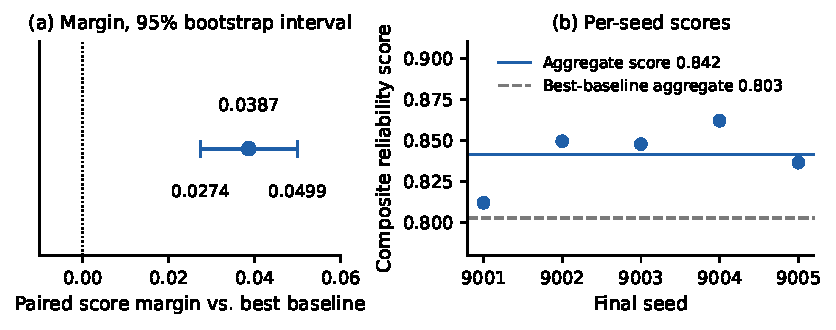
\includegraphics[width=0.88\textwidth]{figures/final_comparison.pdf}
\caption{Sealed final comparison. (a) Paired score margin of the studied procedure over the best of four baselines with its 95\% bootstrap interval (seeded runs within cases, equal weight over cases). (b) Per-seed final scores of the procedure; horizontal lines mark the procedure's aggregate score and the best-baseline aggregate score, so per-seed dots are compared with an aggregate.}
\label{fig:final}
\end{figure}

\begin{table}[!tbp]
\centering
\caption{Sealed final metrics retained by the evaluator. Gaps are one-sided shortfalls; ``shift'' is descriptive.}
\label{tab:final}
\begin{tabular}{lr}
\toprule
Metric & Value \\
\midrule
Composite score of studied procedure & 0.8416 \\
Composite score of best baseline (identity not retained) & 0.8029 \\
Paired margin (95\% bootstrap interval) & 0.0387 (0.0274, 0.0499) \\
Exchangeable-case marginal under-coverage gap & 0.0017 \\
Worst-slice under-coverage gap (all cases) & 0.0675 \\
Shift-case marginal under-coverage gap & 0.0536 \\
Mean set-size ratio & 0.209 \\
Negative controls passed (fraction; count not retained) & 1.0 \\
Failed episodes & 0 \\
\bottomrule
\end{tabular}
% @evidence[[paper_data.json#final_evaluation.metrics]]
\end{table}

\subsection{Reliability profile and residual failures}
The headline margin should be read together with the residual gaps. On exchangeable cases the mean marginal under-coverage gap is 0.0017, compatible with the finite-sample guarantee; being one-sided and averaged over few seeded runs, it neither tests the guarantee nor shows coverage is tight. The mean set-size ratio is 0.209. The shift-case marginal gap is 0.0536 and the worst-slice gap is 0.0675, so both residual failures are larger than the exchangeable gap by more than an order of magnitude. % @evidence[[paper_data.json#final.metric.shift_coverage_gap]] @evidence[[paper_data.json#final.metric.worst_slice_coverage_gap]]

Because Eq.~\eqref{eq:loss} is linear in the case-mean metrics, the mean loss of 0.1584 decomposes as follows: the set-size term contributes $0.25\times0.209=0.0522$, the slice term $0.25\times0.0675=0.0169$, and the remainder, $0.0893$, is the marginal term, equivalent to a mean clipped marginal gap of $0.179$ in units of $\alpha$ over all cases. % @evidence[[derived/derived_stats.json#final_loss_decomposition]]
This subtraction assumes the evaluator aggregates the components exactly as reported, and $\alpha$ is not retained, so we do not convert the term to a coverage number; that shifted cases dominate it is plausible but cannot be established without per-case results. We do not attribute the residual shift or slice gaps to statistical noise, to the density-ratio estimation, or to a validity failure of the weighting: no gate-level diagnostics are retained.

\begin{figure}[!tbp]
\centering
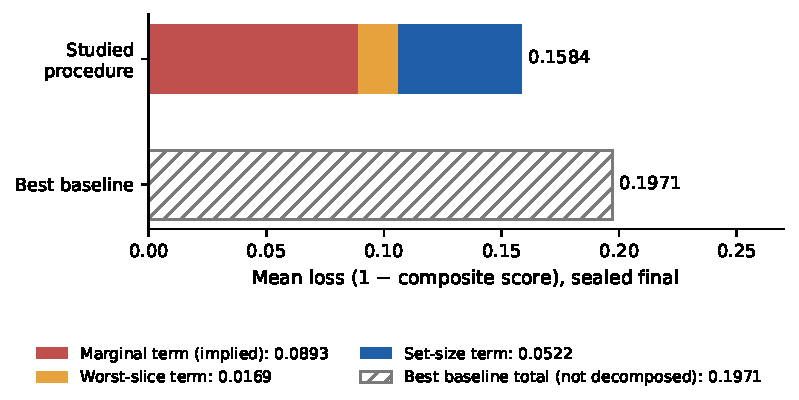
\includegraphics[width=0.66\textwidth]{figures/loss_decomposition.pdf}
\caption{Decomposition of the sealed final mean loss of the studied procedure into the three terms of Eq.~\eqref{eq:loss}. The set-size and worst-slice terms are computed from the retained metrics; the marginal term is the remainder. The best baseline's total loss is shown without decomposition because its components are not retained.}
\label{fig:decomp}
\end{figure}

\subsection{Development-time comparison of nested configurations}
Figure~\ref{fig:variants} shows the three development configurations. Adding the gated weighting to Mondrian LAC (V1 to V2) raised the development score from 0.8683 to 0.9192, reduced the shift-case gap from 0.0613 to 0.0201 and the worst-slice gap from 0.0497 to 0.0376, and left the exchangeable marginal gap unchanged at 0.00028; set size grew from 0.166 to 0.181. % @evidence[[derived/derived_stats.json#variants]]
The per-seed paired differences in score are 0.064, 0.043 and 0.045, all positive, but with three seeds this is descriptive rather than inferential. Because the components are changed together we can say only that the V2 configuration outperformed V1 on these development cases, not which element of the weighting step is responsible.

V3 reproduced V2 in every retained field: score, all six metrics and all three per-seed scores. The V3 source falls back to the V2 path verbatim when its calibration-only gate does not activate, which would give this outcome; but whether the gate was inactive or the quantile-regression thresholds were exercised and rejected is not recorded, so the cause of the tie remains unknown. We therefore report no evidence for or against quantile-regression thresholds.

\begin{figure}[!tbp]
\centering
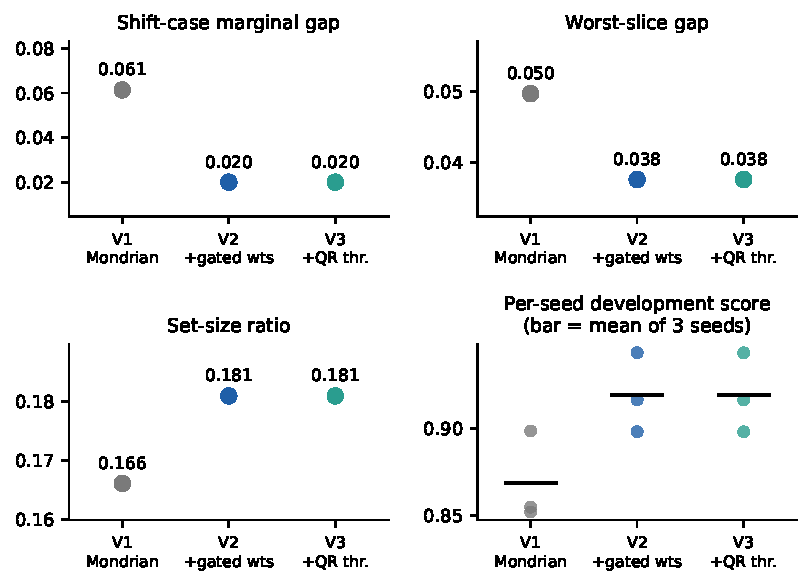
\includegraphics[width=0.72\textwidth]{figures/variant_profile.pdf}
\caption{Development-time comparison of three nested configurations (V1: Mondrian LAC; V2: plus gated weighting, the studied procedure; V3: plus quantile-regression thresholds). Panels show shift-case marginal gap, worst-slice gap, set-size ratio (lower is better) and per-seed scores over seeds 101--103 (higher is better; bar is the mean). V3 coincides with V2 in every retained value. Development cases and seeds differ from the sealed final data.}
\label{fig:variants}
\end{figure}

\subsection{Development-to-final difference}
The development score of the selected procedure (0.9192) is higher than its sealed final score (0.8416), and the final shift gap (0.0536) and set-size ratio (0.209) exceed the development values (0.0201, 0.181). The two evaluations use different seeds and case sets, and sealed cases may be harder; the retained artifacts do not isolate the cause, so we make no statement about selection effects or over-fitting. Only the sealed numbers should be used for conclusions; Table~\ref{tab:devfinal} in the Supplementary Information lists both sets side by side.

\section{Discussion and Limitations}
\paragraph{What the evidence supports.} Within the declared synthetic families and this protocol, the studied procedure has a higher composite score than the best of four standard split-conformal baselines on sealed data, with no failed episode and all negative controls passed. The score margin is the net effect of the evaluator's 0.5/0.25/0.25 weighting; it does not show dominance on each axis, since per-axis baseline values are not retained, and a different weighting could change the ranking. The interval half-width is about 0.011 and the margin is roughly twice the per-seed standard deviation of the procedure's scores (0.019); baseline per-seed scores are not retained, so no seed-level paired effect size can be computed.

\paragraph{What it does not support.} (Table~\ref{tab:inventory} in the Supplementary Information separates available from unknown quantities.)
(i) \emph{Real data.} No real-data run exists; behaviour on classifier outputs from natural datasets is untested.
(ii) \emph{Baseline identity.} Only the best baseline score is retained; we cannot say which baseline it is or how the others compare.
(iii) \emph{Cases and families.} Per-case and per-family results, $\alpha$ and sample sizes of the sealed cases are unknown; the bootstrap interval does not cover variation across case designs.
(iv) \emph{Mechanism.} The comparison among V1--V3 is a design comparison on three seeds and does not isolate the contribution of any single component of the weighting step; V3 provides no information on quantile regression.
(v) \emph{Validity versus statistics.} The residual shift and slice gaps are reported as measured; the diagnostics needed to separate estimation error in the density ratio, small-sample noise and violated assumptions are not available, and candidate-side diagnostics are unverified.
(vi) \emph{Range.} The tested range is limited by the evaluator ($K\le100$, $n_{\mathrm{cal}}\le2000$); nothing is claimed about larger $K$, very small calibration sets, or simplex-valued regression targets.
(vii) \emph{Metric.} One-sided gap metrics do not penalise over-coverage except through set size, and the Mondrian guarantee is conditional on label or confidence bin, not on arbitrary slices, so slice gaps in other partitions are not controlled by theory.

\paragraph{Threats to validity.}
The synthetic generator is one parametric family (Gaussian logits with a true-class signal, heteroscedastic signal strength, a prior tilt and temperature), and the predictor's calibration is not varied independently; real softmax outputs may behave differently. For $K\le10$ the evaluator's slices are classes, which are exactly the Mondrian groups of the studied procedure, so slice-axis results may partly reflect this alignment between method and metric; the class-wise baseline calibrates per label as well, and no per-axis baseline comparison is retained, so any slice-axis advantage is unmeasured. The development score was used to choose the configuration, so development numbers may be optimistic; this was not measured, and the cause of the development-to-sealed drop is not isolated. The sealed evaluation used data disjoint from development by content hash; we have no retained record that it was run only once, and we could not verify which of the two tied configurations (V2 or V3) the sealed metrics belong to beyond their ranking position, so the frozen configuration's identity is not independently verified. Finally, the composite loss multiplies the marginal gap by $1/\alpha$ and clips it, so under-coverage beyond $\alpha$ in a single case is not distinguished; the retained aggregates cannot show whether any case hit this clip.

\paragraph{What would change the conclusion.} The positive margin would be weakened if per-baseline results showed that the best baseline wins on the slice or size axis and loses only on a few shifted cases, or if the sealed cases were mostly shifted. It would be strengthened by per-case margins whose intervals exclude zero and by replication on other case families.

\paragraph{Practical reading.} The residual shift and slice gaps would not have been visible from average coverage and size alone, so we recommend reporting marginal, slice-level and size components separately for every method (Figure~\ref{fig:decomp}), with controls that expose vacuous behaviour.

\section{Conclusion}
We studied a Mondrian least-ambiguous-set conformal procedure with a gated, cross-fitted domain-classifier reweighting step under a multi-axis reliability protocol on synthetic softmax families. On sealed final data it reached a composite score of 0.8416 versus 0.8029 for the best of four standard baselines, a paired margin of 0.0387 with a bootstrap 95\% interval of 0.0274--0.0499, with no failed episodes and all negative controls passed. The same evaluation shows that the procedure does not remove under-coverage under shift (0.0536) or on worst slices (0.0675), and the loss decomposition implies, by subtraction under the evaluator's aggregation, that the marginal term is the largest component (the marginal term is not measured directly, and $\alpha$ and per-case results are unavailable). The conclusions are conditional on the declared synthetic families, on one aggregated best-baseline comparison, and on evaluator-defined weights. Next steps, none yet done, are per-case and per-baseline reporting, ablations isolating the gate and weighting from the Mondrian grouping, gate-activation logging, and evaluation on real classifier outputs.

% IMPORTANT: \clearpage flushes all pending floats before references so that
% body-page counting excludes reference-only pages.  Do NOT remove.
\clearpage
\bibliography{references}
\bibliographystyle{paper}

\clearpage
\appendix
\section{Supplementary Information}

\subsection{Procedure specification}
Table~\ref{tab:hyper} lists the constants of the studied procedure as they appear in its source, and Algorithm-style pseudo-code follows.
% @evidence[[source_evidence/V2/program.py#constants]]

\begin{table}[h]
\centering
\caption{Constants of the studied procedure (from the V2 source; see the identity caveat in Section~\ref{sec:method}).}
\label{tab:hyper}
\begin{tabular}{llr}
\toprule
Component & Constant & Value \\
\midrule
Score & nonconformity & $1-p_k(x)$ \\
Mondrian & class-conditional if & $K\le10$ \\
Mondrian & confidence bins ($K>10$): max bins / min rows per bin & 10 / 80 \\
Margin & pooled / per-group multiplier $z$ & 0.7 / 0.6 \\
Shrinkage & pseudo-count $n_0$ toward pooled threshold & 20 \\
Gate & min. test rows before domain fit & 40 \\
Gate & weights used only if $\beta>$ & $10^{-3}$ \\
Domain classifier & ridge penalty / cross-fit folds / features $d$ & 1 / 2 / 5 \\
Weights & clip range (multiplicative) & $[1/8,\,8]$ \\
Features & standardised clip & $\pm8$ \\
\bottomrule
\end{tabular}
\end{table}

\paragraph{Pseudo-code.}
\emph{Calibrate:} compute scores $s_i=1-p_{y_i}(x_i)$; define groups (label if $K\le10$, else confidence bin); compute per-group margin thresholds $q_g$ and the pooled threshold, with shrinkage; standardise summary features with calibration moments and assign calibration rows to two folds at random.
\emph{Predict (per test chunk):} append the chunk's features; if at least 40 test rows are available, cross-fit the domain classifier on the two folds, compute $\mathrm{LR}$ and $\beta$; if $\beta\le10^{-3}$ or any quantity is non-finite, return $\{k:1-p_k\le q_{g}\}$ with unweighted thresholds; else compute weights $w_i$ (calibration) and $w_j$ (test), form for each test row the weighted group thresholds with $w_j$ at $+\infty$, and return $\{k:1-p_k\le q_{g}(x_j)\}$. The wire protocol limits calibration to two chunks of at most 1000 rows and test data to four chunks.

\subsection{Evaluation protocol details}
The search-time evaluator generates data with the logit model of Section~\ref{sec:setup}; the sealed final plane uses the same scoring, baseline and bootstrap code with different cases and seeds. Slices require at least 30 test points. Controls: C1 permutes calibration labels; C2 permutes test labels when scoring; C3 replaces all probabilities by the uniform vector. In the evaluator, a control episode whose permutation changes fewer than half of the labels is counted as a failed control (\texttt{vacuous\_control}), which invalidates the run. The coverage tolerance for exchangeable cases is $3\sqrt{\alpha(1-\alpha)(1/(n_{\mathrm{cal}}+2)+1/n_{\mathrm{test}})/n_{\mathrm{seeds}}}$. The final evaluator source file is not separately retained, so statements about the final plane rely on the plane-conditional branches of the shared evaluator and on the qualification outcome.
% @evidence[[source_evidence/evaluator/evaluate.py#aggregate]]

\subsection{Full development and per-seed tables}
\begin{table}[h]
\centering
\caption{Development-time metrics for the three nested configurations (seeds 101--103; lower is better for gaps and size ratio, higher for score). Controls passed fraction was 1.0 and failed episodes 0 for all three.}
\label{tab:dev}
\begin{tabular}{lrrrrr}
\toprule
Config. & Score & Exch. gap & Worst-slice gap & Shift gap & Size ratio \\
\midrule
V1 Mondrian LAC & 0.8683 & 0.00028 & 0.0497 & 0.0613 & 0.166 \\
V2 + gated weighting & 0.9192 & 0.00028 & 0.0376 & 0.0201 & 0.181 \\
V3 + QR thresholds & 0.9192 & 0.00028 & 0.0376 & 0.0201 & 0.181 \\
\bottomrule
\end{tabular}
% @evidence[[derived/derived_stats.json#variants]]
\end{table}

\begin{table}[h]
\centering
\caption{Per-seed scores. Final seeds are sealed-evaluation runs (duration in seconds; what the durations cover is not recorded); development seeds are for V1/V2 (V3 identical to V2).}
\label{tab:seeds}
\begin{tabular}{lrrr}
\toprule
Seed & Score & Seed (dev.) & V1 / V2 score \\
\midrule
9001 & 0.8121 (7.6 s) & 101 & 0.8519 / 0.9163 \\
9002 & 0.8495 (4.3 s) & 102 & 0.8547 / 0.8980 \\
9003 & 0.8478 (4.3 s) & 103 & 0.8984 / 0.9433 \\
9004 & 0.8620 (4.3 s) & & \\
9005 & 0.8365 (4.3 s) & & \\
\bottomrule
\end{tabular}
% @evidence[[paper_data.json#final_evaluation.evaluation_evidence.episodes]]
\end{table}

\begin{table}[h]
\centering
\caption{The selected procedure on development data (seeds 101--103) and on sealed final data (seeds 9001--9005). Different cases and seeds; shown side by side for transparency, not as a paired comparison.}
\label{tab:devfinal}
\begin{tabular}{lrr}
\toprule
Metric & Development & Sealed final \\
\midrule
Composite score & 0.9192 & 0.8416 \\
Exchangeable marginal gap & 0.0003 & 0.0017 \\
Worst-slice gap & 0.0376 & 0.0675 \\
Shift-case marginal gap & 0.0201 & 0.0536 \\
Set-size ratio & 0.181 & 0.209 \\
\bottomrule
\end{tabular}
% @evidence[[derived/derived_stats.json#variants]] @evidence[[paper_data.json#final_evaluation.metrics]]
\end{table}

\subsection{Derived quantities}
\begin{itemize}
\item Full-set score: $1-(0.5\cdot0+0.25\cdot0+0.25\cdot1)=0.75$ for every case (analytic).
\item Relative loss reduction: $(0.1971-0.1584)/0.1971=19.6\%$. % @evidence[[derived/derived_stats.json#final_loss_decomposition]]
\item Expected one-sided shortfall factor: $f(0)=0.399$, $f(0.6)=0.169$, $f(0.7)=0.143$. % @evidence[[derived/derived_stats.json#margin_constants]]
\item Development paired differences V2$-$V1: 0.064, 0.043, 0.045 (mean 0.051); V3$-$V2: 0, 0, 0.
\end{itemize}

\subsection{Reproducibility and what is not retained}

\begin{table}[htbp]
\centering
\caption{Evidence inventory for the sealed final evaluation.}
\label{tab:inventory}
\begin{tabular}{p{0.46\textwidth}p{0.42\textwidth}}
\toprule
Available & Not retained (unknown) \\
\midrule
Aggregate score, best-baseline aggregate score, paired margin and bootstrap interval & Identity and individual scores of the four baselines \\
Five per-seed scores; failed-episode count; control pass fraction & Per-case and per-family results; which cases drive shift and slice gaps \\
Exchangeable, shift, worst-slice and size-ratio aggregates & $\alpha$, $K$ and sample sizes of the sealed cases \\
Source of the studied procedure and of the evaluator code & Gate-activation frequency; cause of the development-to-final drop; cause of the V3--V2 tie \\
\bottomrule
\end{tabular}
\end{table}

The figures and derived numbers are produced by \texttt{scripts/build\_figures.py} and \texttt{scripts/derive\_stats.py} from the evaluator's recorded outputs; the candidate sources and the evaluator source are included in the artifact bundle, and the evaluator requires NumPy 2.2.6 (SciPy is optional in the candidate). Development seeds are 101--103 and final seeds 9001--9005; the final runs took 4--8 seconds each. The sealed final case manifest and the per-baseline results are not retained, so the final numbers cannot be regenerated from the retained files and must be read as evaluator-reported values. No external dataset was used (so no data licence applies), and no real-data experiment was run, including the CIFAR-10 option offered by the task. Bibliographic descriptions in Section~\ref{sec:related} rely on titles and venues in the retrieval metadata only. Citations to the split/Mondrian, score-function, covariate-shift and compositional-data sources (Section~\ref{sec:related}) support background statements only; the retrieval metadata record titles, venues and years, and the implementation details of the baselines and of the studied procedure come from the evaluator and candidate sources, not from those papers.

\subsection{LLM Usage}
Large language models were used in this work in two roles. First, an LLM-driven research agent proposed, implemented and evaluated three candidate configurations (V1--V3 here) against the evaluator and wrote the initial analysis. Second, an LLM drafted this manuscript from the evaluator outputs and the retained sources. All reported numbers are copied or arithmetically derived from evaluator outputs.

\end{document}
